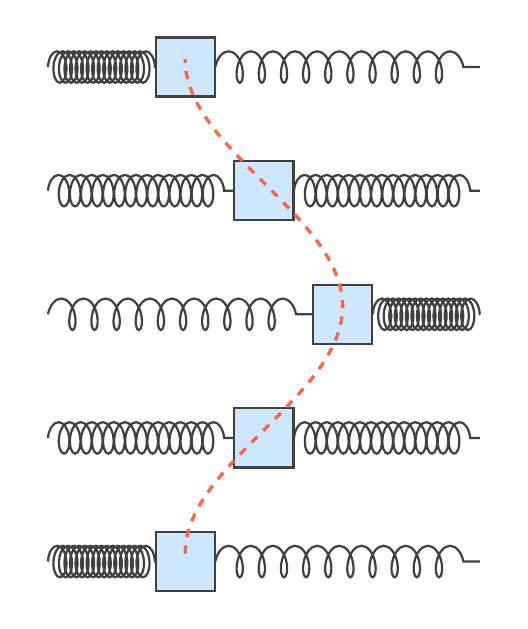
\begin{tikzpicture}[scale=0.5, transform shape]

\tikzstyle{M1}=[rectangle,draw=none,fill=DodgerBlue!22,minimum size=1.5cm,thick]
\tikzstyle{spring}=[darkgray,thick,decorate,decoration={aspect=0.5, segment length=2, amplitude=2mm,coil}]
\tikzstyle{ground}=[fill=white, thick, minimum width=0.75cm,minimum height=2cm]

\begin{scope}
\node[M1,yshift=-0.2cm,xshift=-2cm,draw=darkgray,thick](zm1){};
\node[ground,minimum width=0.5cm,xshift=-5.75cm,yshift=-0.2cm](zLWall){};
\node[ground,minimum width=0.5cm,xshift=5.75cm,yshift=-0.2cm](zRWall){};
\draw [spring](zLWall.east) -- (zm1.west);
\draw[spring, segment length=8](zm1.east) -- (zRWall.west);
% \node[above] at (6,0) {\large $t=0$};
\end{scope}

\begin{scope}[yshift=-3.14cm]
\node[M1,yshift=-0.2cm,xshift=0cm,draw=darkgray,thick](qm1){};
\node[ground,minimum width=0.5cm,xshift=-5.75cm,yshift=-0.2cm](qLWall){};
\node[ground,minimum width=0.5cm,xshift=5.75cm,yshift=-0.2cm](qRWall){};
\draw [spring,segment length=4](qLWall.east) -- (qm1.west);
\draw[spring, segment length=4](qm1.east) -- (qRWall.west);
% \node[above] at (6,0) {\large $t=\nicefrac{1}{4}T$};
\end{scope}

\begin{scope}[yshift=-6.28cm]
\node[M1,yshift=-0.2cm,xshift=2cm,draw=darkgray,thick](jm1){};
\node[ground,minimum width=0.5cm,xshift=-5.75cm,yshift=-0.2cm](jLWall){};
\node[ground,minimum width=0.5cm,xshift=5.75cm,yshift=-0.2cm](jRWall){};
\draw [spring, segment length=8](jLWall.east) -- (jm1.west);
\draw[spring, segment length=2](jm1.east) -- (jRWall.west);
% \node[above] at (6,0) {\large $t=\nicefrac{1}{2}T$};
\end{scope}

\begin{scope}[yshift=-9.42cm]
\node[M1,yshift=-0.2cm,xshift=0cm,draw=darkgray,thick](ym1){};
\node[ground,minimum width=0.5cm,xshift=-5.75cm,yshift=-0.2cm](yLWall){};
\node[ground,minimum width=0.5cm,xshift=5.75cm,yshift=-0.2cm](yRWall){};
\draw [spring,segment length=4](yLWall.east) -- (ym1.west);
\draw[spring, segment length=4](ym1.east) -- (yRWall.west);
% \node[above] at (6,0) {\large $t=\nicefrac{3}{4}T$};
\end{scope}

\begin{scope}[yshift=-12.56cm]
\node[M1,yshift=-0.2cm,xshift=-2cm,draw=darkgray,thick](om1){};
% \node[below] at (atrack.south){};
\node[ground,minimum width=0.5cm,xshift=-5.75cm,yshift=-0.2cm](oLWall){};
\node[ground,minimum width=0.5cm,xshift=5.75cm,yshift=-0.2cm](oRWall){};
\draw [spring](oLWall.east) -- (om1.west);
\draw[spring, segment length=8](om1.east) -- (oRWall.west);
% \node[above] at (6,0) {\large $t=T$};
\end{scope}

% \path[very thick, red] (zm1.center) edge [dotted, sin] (qm1.center);
% \path[very thick, red] (qm1.center) edge [dotted, cos] (jm1.center);
% \draw[ultra thick, red, bend right] (zm1) sin (qm1);
% \draw[ultra thick, blue] (jm1) sin (qm1);
% \draw[ultra thick, red] (jm1) sin (ym1);
% \draw[ultra thick, blue] (ym1) cos (om1);

\draw[very thick, Tomato, dashed,yshift=-6.28cm, rotate=90] (-6.28,2) cos (-3.14,0) sin (0,-2) cos (3.14,0) sin (6.28,2);

\end{tikzpicture}


